\chapter{Mixed Strategies}

\section{Introduction and Motivation}
In some games (e.g., striker vs. goalkeeper, Rock-Paper-Scissors), a pure strategy equilibrium does not exist. If the striker knows the goalkeeper's deterministic action, they can always win. The real equilibrium requires randomness, or more precisely, unpredictability.

\section{Formal Definitions}

\subsection{Mixed Strategy and Representations}
\begin{definition}[Mixed Strategy]
A mixed strategy of player $i$ is a probability measure on their action set $X_i$.
\begin{itemize}
    \item If $X_i$ is finite, it is a vector $\sigma_i \in \Delta(X_i) = \{ p \in [0,1]^{|X_i|} : \sum p_k = 1 \}$.
    \item If $X_i$ is continuous (compact), it is a regular probability measure $\mu_i$ on the Borel sigma-algebra of $X_i$.
\end{itemize}
\end{definition}

\begin{definition}[Specific Vocabulary]
\begin{itemize}
    \item \textbf{Pure Strategy (Dirac):} A pure strategy $a_i \in X_i$ can be seen as a degenerate mixed strategy that puts all the weight on $a_i$. It is denoted $\delta_{a_i}$ (Dirac measure).
    \item \textbf{Totally Mixed Strategy:} A mixed strategy $\sigma_i$ is said to be \textbf{totally mixed} if its support is complete, i.e., if it assigns a strictly positive probability to each possible pure action: $\forall x_i \in X_i, \sigma_i(x_i) > 0$.
\end{itemize}
\end{definition}

\paragraph{Triple Representation:}
A mixed strategy can be viewed in three complementary ways:
\begin{enumerate}
    \item \textbf{Geometric:} A point in the simplex $\Delta(X_i)$.
    \item \textbf{Functional:} A mass function (discrete case) or density function.
    \item \textbf{Measure:} A probability measure $\mu$ on the set of Borel sets.
\end{enumerate}

\begin{center}
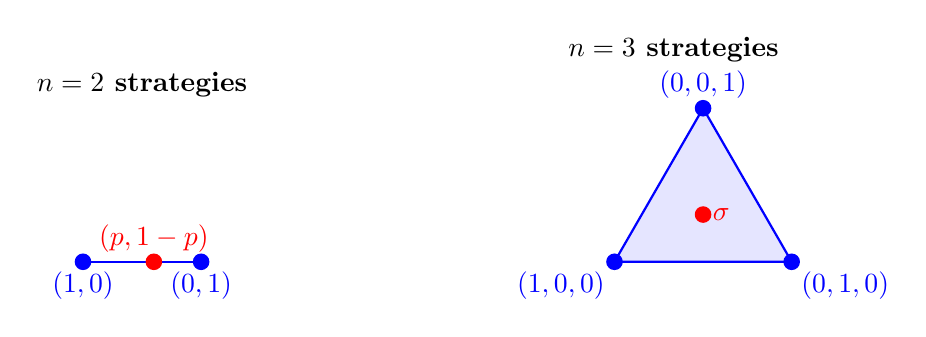
\begin{tikzpicture}[scale=1.5]
    % Simplex for n=2 (segment)
    \begin{scope}[shift={(-2.5,0)}]
        \node at (0.5, 1.5) {\textbf{$n=2$ strategies}};
        \draw[thick, blue] (0,0) -- (1,0);
        \fill[blue] (0,0) circle (2pt) node[below] {$(1,0)$};
        \fill[blue] (1,0) circle (2pt) node[below] {$(0,1)$};
        \fill[red] (0.6,0) circle (2pt);
        \node[red, above] at (0.6,0) {$(p, 1-p)$};
    \end{scope}
    
    % Simplex for n=3 (triangle)
    \begin{scope}[shift={(2,0)}]
        \node at (0.5, 1.8) {\textbf{$n=3$ strategies}};
        \coordinate (A) at (0,0);
        \coordinate (B) at (1.5,0);
        \coordinate (C) at (0.75,1.3);
        \draw[thick, blue, fill=blue!10] (A) -- (B) -- (C) -- cycle;
        \fill[blue] (A) circle (2pt) node[below left] {$(1,0,0)$};
        \fill[blue] (B) circle (2pt) node[below right] {$(0,1,0)$};
        \fill[blue] (C) circle (2pt) node[above] {$(0,0,1)$};
        % Interior point
        \fill[red] (0.75,0.4) circle (2pt);
        \node[red, right] at (0.75,0.4) {$\sigma$};
    \end{scope}
\end{tikzpicture}
\captionof{figure}{The simplex $\Delta(X_i)$: segment for 2 strategies, triangle for 3.}
\end{center}

\subsection{Mixed Extension}
The mixed extension is the "new" game where players choose probability distributions.

\begin{definition}[Expected Payoff and Independence Assumption]
Player $i$'s payoff in the mixed extension is defined as the \textbf{expected payoff} with respect to the product law of individual strategies.
\textbf{Fundamental Assumption:} Players' random choices are assumed to be \textbf{independent}. The mixed strategy profile is therefore the product measure $P = \sigma_1 \otimes \sigma_2 \otimes \dots \otimes \sigma_n$ on the space $X = \prod X_i$.

\textbf{Integral Formulation:}
$$\tilde{u}_i(\sigma_1, \dots, \sigma_n) = \int_{X_1} \dots \int_{X_n} u_i(x_1, \dots, x_n) d\sigma_1(x_1) \dots d\sigma_n(x_n)$$

\subsection{Mixed strategies in continuous universe}
If the action set $X_i$ is a metric space (e.g., $[0,1]$), a mixed strategy $\sigma_i$ is a \textbf{Borel probability measure} on $X_i$.
We denote $\Delta(X_i)$ the set of these measures. The expected payoff is then:
\[ u_i(\sigma_1, \dots, \sigma_n) = \int_{X_1} \dots \int_{X_n} u_i(x_1, \dots, x_n) d\sigma_1(x_1) \dots d\sigma_n(x_n) \]
In the finite case:
$$\tilde{u}_i(\sigma) = \sum_{x \in X} u_i(x) \left( \prod_{j \in N} \sigma_j(x_j) \right)$$
\end{definition}

\section{Nash Equilibrium in Mixed Strategies}

\subsection{Existence and Link to Pure Strategies}
\begin{theoreme}[Nash, 1950]
Every finite game has at least one Nash equilibrium in mixed strategies.
\end{theoreme}

\begin{proposition}[Pure/Mixed Relation]
The mixed extension is a coherent generalization.
If $x^* = (x^*_1, \dots, x^*_n)$ is a pure strategy Nash equilibrium of the original game, then the profile of Dirac measures $(\delta_{x^*_1}, \dots, \delta_{x^*_n})$ is a Nash equilibrium of the mixed extension.
\end{proposition}

\subsection{Indifference Principle (Fundamental)}
This is the main tool for calculating mixed equilibria.

\begin{proposition}[Indifference Principle]
Let $\sigma^*$ be a mixed Nash equilibrium. For any player $i$, any pure action $x_i$ belonging to the \textbf{support} of their strategy (i.e., played with positive probability $\sigma^*_i(x_i) > 0$) must yield the same expected payoff:
$$u_i(x_i, \sigma^*_{-i}) = \max_{a_i \in X_i} u_i(a_i, \sigma^*_{-i}) = \tilde{u}_i(\sigma^*)$$
In other words, the player is \textbf{indifferent} between all the actions they actually play. Unplayed actions yield a lower or equal payoff.
\end{proposition}

\begin{proof}[Proof by contradiction]
Suppose there exists an action $a$ in the support of $\sigma_i^*$ such that $u_i(a, \sigma^*_{-i}) < M$, where $M = \max_{z} u_i(z, \sigma^*_{-i})$.
\begin{enumerate}
    \item Let $b$ be an action that achieves the maximum $M$.
    \item Construct a new strategy $\sigma'_i$ by transferring weight (probability) $p_a > 0$ from the "mediocre" action $a$ to the "optimal" action $b$.
    \item The expected payoff becomes:
    \begin{align*}
    \tilde{u}_i(\sigma'_i, \sigma^*_{-i}) &= \tilde{u}_i(\sigma^*_i, \sigma^*_{-i}) - p_a \underbrace{u_i(a, \sigma^*_{-i})}_{< M} + p_a \underbrace{u_i(b, \sigma^*_{-i})}_{M} \\
    &> \tilde{u}_i(\sigma^*_i, \sigma^*_{-i})
    \end{align*}
    \item Since $u_i(b) > u_i(a)$, we have $\tilde{u}_i(\sigma') > \tilde{u}_i(\sigma^*)$.
\end{enumerate}
This contradicts the fact that $\sigma^*$ was a best response (Nash equilibrium). Therefore, all actions in the support must yield the maximum $M$.
\end{proof}

\section{Topological and Measure Foundations}
This section details the rigorous mathematical framework necessary for infinite games.

\begin{itemize}
    \item \textbf{Borel Sigma-Algebra:} Each action space $X_i$ (assumed compact metric) is equipped with its Borel sigma-algebra $\mathcal{B}(X_i)$, the smallest $\sigma$-algebra containing all open sets.
    \item \textbf{Regular Measures:} We consider the space $\mathcal{M}(X_i)$ of regular probability measures (any measure on a compact metric space is regular, i.e., internally approximable by compacts and externally by open sets).
    \item \textbf{Weak-* Topology:} The convergence of a sequence of strategies $\mu_n \to \mu$ is defined by the convergence of integrals against any continuous test function $f$:
    $$\forall f \in C^0(X_i, \mathbb{R}), \quad \int_{X_i} f d\mu_n \to \int_{X_i} f d\mu$$
    \item \textbf{Semi-norms:} This topology is induced by the family of semi-norms $P_f(\mu) = |\int f d\mu|$.
\end{itemize}

\begin{theoreme}[Weak Compactness]
If $X_i$ is compact metric, then the set of mixed strategies $\Delta(X_i)$ is compact for the weak-* topology.
\end{theoreme}
It is this theorem, combined with the linearity (thus quasi-concavity) of expected payoffs, that allows applying Glicksberg's theorem to prove the existence of equilibria in continuous games.

\section{Classic Examples}

\begin{exemple}[Detailed 2x2 Calculation Example]
Consider the following game, where Player 1 (rows) chooses between $X$ and $Y$, and Player 2 (columns) between $x$ and $y$.
\begin{center}
\begin{tabular}{c|c|c}
 & $x$ ($q$) & $y$ ($1-q$) \\ \hline
$X$ ($p$) & (2, 1) & (0, 0) \\ \hline
$Y$ ($1-p$) & (0, 0) & (1, 2)
\end{tabular}
\end{center}
Player 1 plays $X$ with probability $p$, Player 2 plays $x$ with probability $q$.

\textbf{Calculation for Player 1 (Indifference):}
For P1 to be willing to mix (play randomly), they must be indifferent between $X$ and $Y$. Their expected payoffs must be equal:
\[ E[U_1(X, \sigma_2)] = E[U_1(Y, \sigma_2)] \]
\[ q \cdot 2 + (1-q) \cdot 0 = q \cdot 0 + (1-q) \cdot 1 \]
\[ 2q = 1 - q \implies 3q = 1 \implies q = 1/3 \]

\textbf{Calculation for Player 2 (Indifference):}
Similarly, P2 must be indifferent between $x$ and $y$:
\[ E[U_2(\sigma_1, x)] = E[U_2(\sigma_1, y)] \]
\[ p \cdot 1 + (1-p) \cdot 0 = p \cdot 0 + (1-p) \cdot 2 \]
\[ p = 2(1 - p) \implies p = 2 - 2p \implies 3p = 2 \implies p = 2/3 \]

\textbf{Conclusion:} The unique mixed strategy Nash equilibrium is the profile $((p=2/3), (q=1/3))$.
Graphically, the best response correspondences intersect at this point $(2/3, 1/3)$ in the probability square.
\end{exemple}

\begin{exemple}[Chicken Game]
P1 Indifference: $-4q + (1-q) = -q \implies q = 1/4$.
\end{exemple}
